\documentclass{article}

\usepackage{amsmath}
\usepackage{amssymb}
\usepackage{upgreek}
\usepackage{graphicx}
\usepackage[font={footnotesize,it}]{caption}
%\usepackage[margin=0.5in]{geometry} %remove comment after todonotes are dealt with
%\usepackage[textwidth=1.5in]{todonotes}
%\usepackage{parskip}

\title{Research Proposal}
\author{Nitish Thatte}

\begin{document}
\maketitle

\section*{Introduction}


We wish to control a quadrupedal robot with the following per leg linear relationship between leg rotation speed and generated force

\begin{equation}
	F_i = A_i + B_i^+ \omega_i^+ + B_i^- \omega_i^-
\end{equation}

Where $i \in \{1,2,3,4\}$ corresponds to one of the four legs and $\omega_i^+$ and $\omega_i^-$ are the leg velocities for the upwards and downwards parts of the trajectories respectively. Our goal is to control the height, pitch, and roll of the robot. We can write the Newton-Euler equations for these degrees of freedom:

\begin{align}
	m \ddot{y} &= \sum_{i=1}^4 (A_i + B_i^+ \omega_i^+ + B_i^- \omega_i^-) - mg \\
	I_x \ddot{\theta} &= l_x \left[ \sum_{i = \{1,2\}} \left(A_i + B_i^+ \omega_i^+ + B_i^- \omega_i^- \right) - \sum_{i = \{3,4\}} \left(A_i + B_i^+ \omega_i^+ + B_i^- \omega_i^- \right) \right] \\
	I_z \ddot{\phi} &= l_z \left[ \sum_{i = \{1,4\}} \left(A_i + B_i^+ \omega_i^+ + B_i^- \omega_i^- \right) - \sum_{i = \{2,3\}} \left(A_i + B_i^+ \omega_i^+ + B_i^- \omega_i^- \right) \right]
\end{align}

Where $m$ is the mass of the robot, $I_x$ and $I_z$ are the moments of inertia about the $x$ and $z$-axes respectively, and $l_x$ and $l_z$ are the distances to the center of mass in the $x$ and $z$ directions respectively. In matrix form these equations are 

\begin{equation}
	\begin{bmatrix} m & 0 & 0 \\ 0 & I_{x} & 0 \\ 0 & 0 & I_{z} \end{bmatrix} 
	\begin{bmatrix} \ddot{y} \\ \ddot{\theta} \\ \ddot{\phi} \end{bmatrix} = 
	\begin{bmatrix} \sum A_i - mg \\ \bar{L}_x^T \bar{A} \\ \bar{L}_z^T \bar{A} \end{bmatrix} +
	\begin{bmatrix} \bar{B}_+^T & \bar{B}_-^T \\ \bar{B}_+^T \hat{L}_x & \bar{B}_-^T \hat{L}_x \\ \bar{B}_+^T \hat{L}_z & \bar{B}_-^T \hat{L}_z \end{bmatrix} 
	\begin{bmatrix} \bar{\omega}^+ \\ \bar{\omega}^- \end{bmatrix}
	\label{eq:Newton-Euler}
\end{equation}

Where 

\begin{align}
	\bar{L}_x &= l_x \begin{bmatrix} 1 \\ 1 \\ -1 \\ -1 \end{bmatrix} \\
	\hat{L}_x &= l_x \begin{bmatrix} 1 & 0 & 0 & 0\\ 0 & 1 & 0 & 0 \\ 0 & 0 & -1 & 0\\ 0 & 0 & 0 & -1 \end{bmatrix} \\
	\bar{L}_z &= l_z \begin{bmatrix} 1 \\ -1 \\ -1 \\ 1 \end{bmatrix} \\
	\hat{L}_z &= l_z \begin{bmatrix} 1 & 0 & 0 & 0\\ 0 & -1 & 0 & 0 \\ 0 & 0 & -1 & 0\\ 0 & 0 & 0 & 1 \end{bmatrix}
\end{align}

We can write equation~\ref{eq:Newton-Euler} compactly as

\begin{equation}
	M \ddot{\bar{x}} = A + B \bar{\omega}
	\label{eq:Newton-Euler-Mat}
\end{equation}

Where $\bar{x} = [y, \ \theta, \ \phi]^T$ is the state of the robot and $\bar{\omega} = [\bar{\omega}^+, \ \bar{\omega}^-]^T$.

In order to achieve a desired state $x_0$ we employ virtual model control using a virtual spring. Therefore, our desired dynamics are

\begin{equation}
	\ddot{\bar{x}} = K_p (\bar{x}_0 - \bar{x})
	\label{eq:virtSpring}
\end{equation}

We wish to find a $\bar{\omega}$ that will achieve the above dynamics so we will now solve for a suitable $\bar{\omega}$. Plugging equation~\ref{eq:virtSpring} into equation~\ref{eq:Newton-Euler-Mat} and rearranging yields

\begin{equation}
	B \bar{\omega} = M K_p (\bar{x}_0 - \bar{x}) - A
\end{equation}

We cannot simply invert $B$ in order to solve for $\bar{\omega}$ as it is not a square matrix.  Rather, in our case the size of $B$ is $3 \times 8$. Therefore, there are potentially an infinite set of $\bar{\omega}$s that will satisfy our desired dynamics. In order to find one suitable $\bar{\omega}$, we can formulate a constrained optimization that will provide the solution closest to a specified $\bar{\omega}_0$ that adheres to our virtual model:

\begin{equation}
	\bar{\omega} = \arg \min \frac{1}{2} (\bar{\omega} - \bar{\omega}_0)^T (\bar{\omega} - \bar{\omega}_0) \textrm{~such that~} B \bar{\omega} = M K_p (\bar{x}_0 - \bar{x}) - A
\end{equation}

We can solve the above optimization by incorporating the constraint into the cost function using the Lagrange Multipliers Method.

\begin{equation}
	\bar{\omega} = \arg \min \frac{1}{2} (\bar{\omega} - \bar{\omega}_0)^T (\bar{\omega} - \bar{\omega}_0) + \bar{\lambda}^T  (M K_p (\bar{x}_0 - \bar{x}) - A - B \bar{\omega})
\end{equation}

The solution to the above minimization is

\begin{equation}
	\bar{\omega} = B^\dagger [M K_p (\bar{x}_0 - \bar{x}) - A] + (I - B^\dagger B) \bar{\omega}_0
	\label{eq:controller}
\end{equation}

Where $B^\dagger = B^T (B B^T)^{-1}$ is the Moore-Penrose pseudoinverse of $B$ and $I - B^\dagger B$ is the nullspace projector of $B$. Multiplication of the nullspace projector by $\bar{\omega}_0$ will return as much of $\bar{\omega}_0$ as possible while adhering to our desired spring-like dynamics.

In order to implement the high-level controller for robot-state derived above, we will also need a lower-level of control to guide each leg to along the trajectories specified by $\bar{\omega}$. To do this, we turn to a closed-loop central pattern generator (CPG) network.

\section*{CPG Network}

\todo{This section needs a bit more introduction. I added a small transition to the topic as my last sentence}
Equations for one node in the network.

\begin{align}\label{eq:one_node}
	\dot \phi_i &= \omega_{b} + \sum_{j \neq i} k_{ij} \sin \left( \phi_j - \phi_i - \tilde{\varphi}_{ij} \right ) + \zeta_i\\
	\Gamma_i    &= A \cos(\phi_i)
\end{align}

where $\phi_i$ is the phase of \textit{i}th node, $k_{ij}$ and $\tilde{\varphi}_{ij}$ are coupling gain and desired phase lag between $i$th and $j$th node in the network. $\zeta_i$ is the input force for the $i$th node, which is determined by the controller discussed in the previous section. Amplitude and frequency, $A$ and $\omega$ are equal for all nodes in the system. And finally, $\Gamma_i$ is the output of node $i$ and will be used as the desired trajectory for the $i$th motor.

In our network, $i$ can be any of four actuators on the robot, namely \textit{front-right}, \textit{front-left}, \textit{hind-right}, and  \textit{hind-left}, as shown in figure below, respectively nodes 1 to 4.

\begin{figure}[thpb]
	\centering
		\centering
		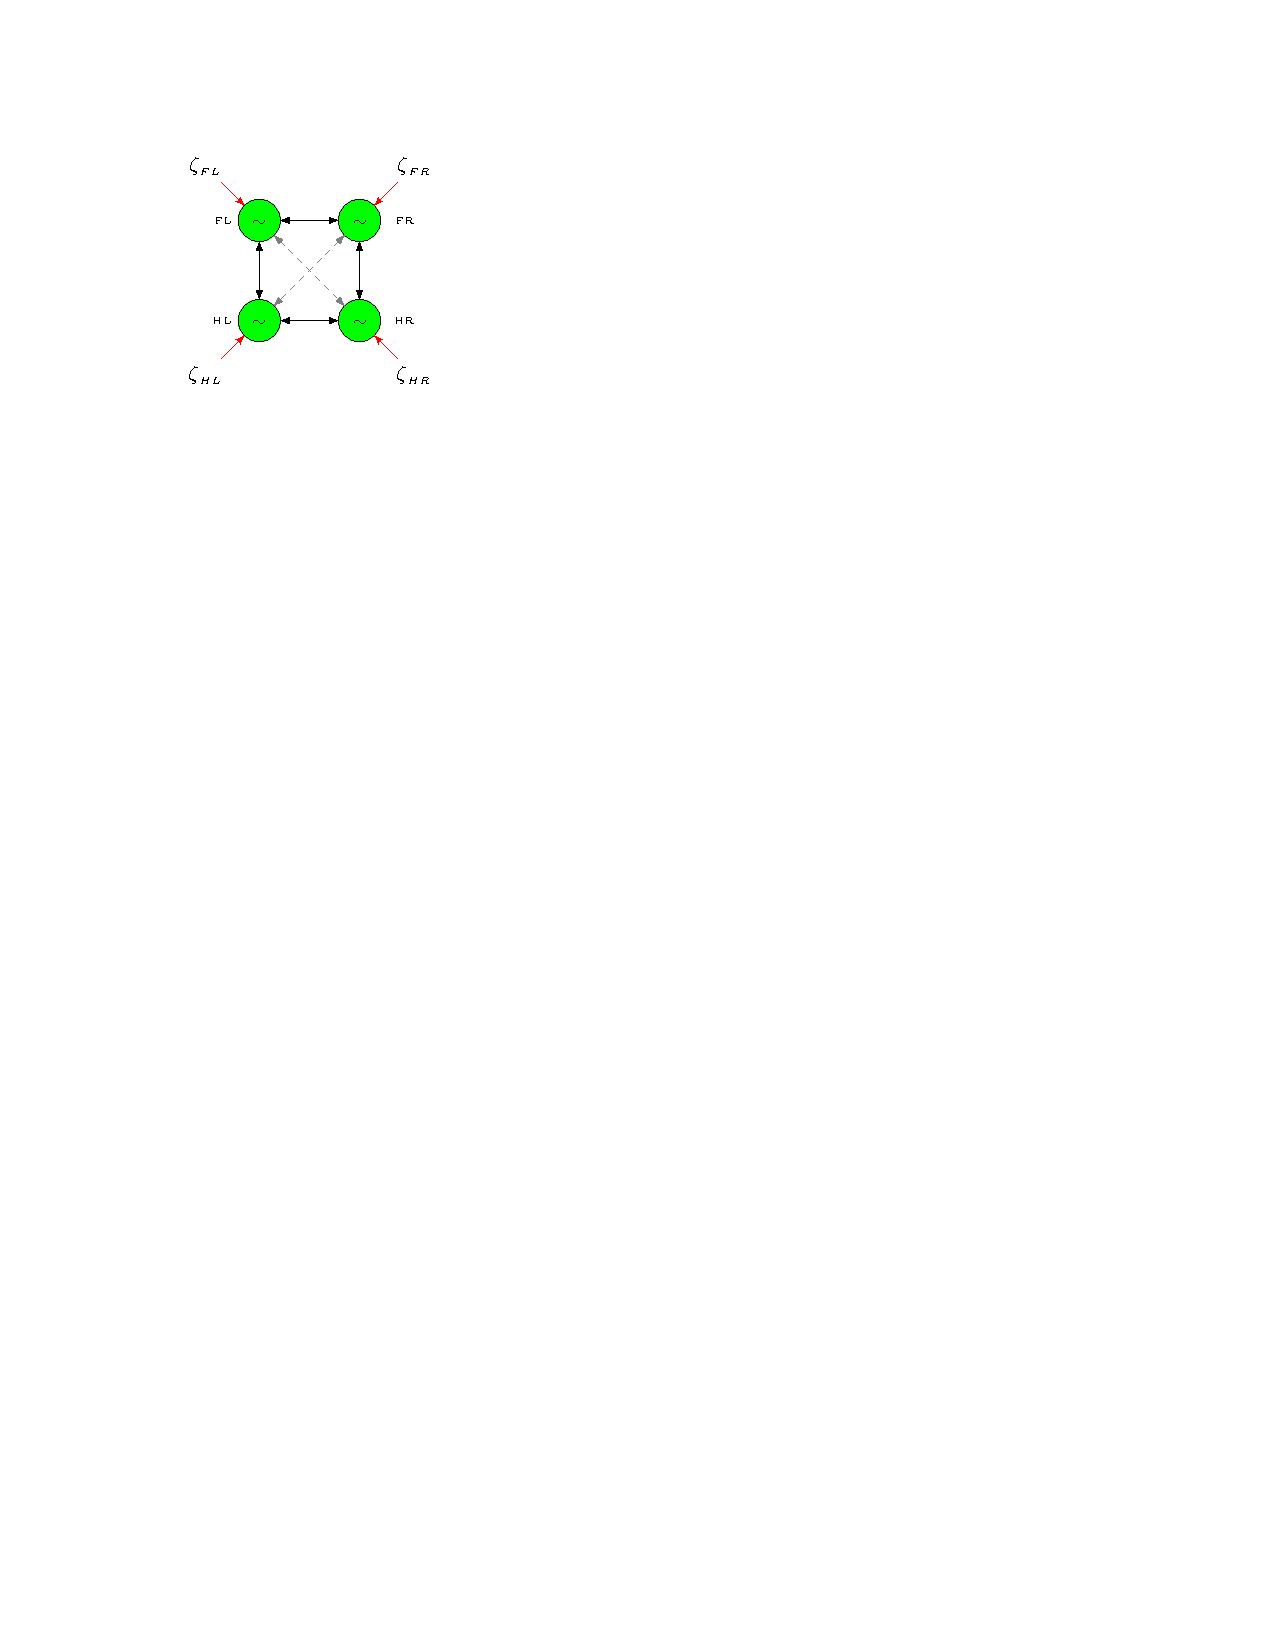
\includegraphics[scale = 0.95]{schema_cropped.pdf}
		\centering
		\caption{CPG network}
		\label{fig:CPG_Network}
\end{figure}

In the CPG network, $\varphi_{ij}$ determines the gait for robot. In order to ensure moments on the body are balanced we chose the the trot gait. Therefore, the phase lags in matrix form are:

\begin{equation}
	\tilde{\Phi} = [\tilde{\varphi}_{ij}]=\left[ \begin{array}{rrrr}
	0    & \pi & \pi  & 0   \\
	-\pi & 0   & 0    & \pi  \\
	-\pi & 0   & 0    & \pi   \\
	0    & -\pi&-\pi  & 0 
	\end{array} \right]
\end{equation}
	
This matrix is a skew-symmetric because of the phase lag property:

\begin{equation}
	\tilde{\varphi}_{ij} = - \tilde{\varphi}_{ji}
\end{equation}

As illustrated in Figure~\ref{fig:CPG_Network}, where dashed-grey line means coupling gain of zero, we are not using fully connected network. \todo{Can you explain why we are't using a fully connected network here} We are using the same coupling gains in the network. Therefore, the matrix representation of the coupling gains is:
 
\begin{equation}
	\upkappa = [k_{ij}]=\left[ \begin{array}{rrrr}
	0 & k & k & 0  \\
	k & 0 & 0 & k  \\
	k & 0 & 0 & k  \\
	0 & k & k & 0 
	\end{array} \right]
\end{equation}

The differential equations for our CPG-Network are as follows:

\begin{align}\label{eq:cpg_net}
	\dot\phi_1&=\omega_{b} + k\sin \left(\phi_2-\phi_1-\tilde{\varphi}_{12}\right)+k\sin\left(\phi_3-\phi_1-\tilde{\varphi}_{13}\right)+ \zeta_1\\
 	\dot\phi_2&=\omega_{b} + k\sin \left(\phi_1-\phi_2-\tilde{\varphi}_{21}\right)+k\sin\left(\phi_4-\phi_2-\tilde{\varphi}_{24}\right)+ \zeta_2\\
 	\dot\phi_3&=\omega_{b} + k\sin \left(\phi_1-\phi_3-\tilde{\varphi}_{31}\right)+k\sin\left(\phi_4-\phi_3-\tilde{\varphi}_{34}\right)+ \zeta_3\\
	\dot\phi_4&=\omega_{b} + k\sin \left(\phi_2-\phi_4-\tilde{\varphi}_{42}\right)+k\sin\left(\phi_3-\phi_4-\tilde{\varphi}_{43}\right)+ \zeta_4
\end{align}

Using the following linear transformation, $\varphi_{ij} = \phi_j - \phi_i - \tilde{\varphi}_{ij}$, and knowing that $\dot{\tilde{\varphi}}_{ij} = 0$ and $\varphi_{ij} = - \varphi_{ji}$, we arrive at the differential equations in phase lags coordination: \todo{Something seems wrong about the ending of this sentence. I'm not sure what its trying to say. Do you mean phase lag coordinates?}

\begin{align}\label{eq:cpg_net2}
	\dot\phi_1&=\omega_{b} + k\sin \left(\varphi_{12}\right)+k\sin\left(\varphi_{13}\right)+ \zeta_1\\
 	\dot\phi_2&=\omega_{b} + k\sin \left(\varphi_{21}\right)+k\sin\left(\varphi_{24}\right)+ \zeta_2\\
 	\dot\phi_3&=\omega_{b} + k\sin \left(\varphi_{31}\right)+k\sin\left(\varphi_{34}\right)+ \zeta_3\\
	\dot\phi_4&=\omega_{b} + k\sin \left(\varphi_{42}\right)+k\sin\left(\varphi_{43}\right)+ \zeta_4
\end{align}

\begin{align}
	\dot\varphi_{12}&= -2k\sin \left(\varphi_{12}\right)-k\sin\left(\varphi_{13}\right)+ k\sin\left(\varphi_{24}\right) + \zeta_2-\zeta_1 \label{eq:cpg_net3_1}\\
	\dot\varphi_{13}&= -2k\sin \left(\varphi_{13}\right)-k\sin\left(\varphi_{12}\right)+ k\sin\left(\varphi_{34}\right) + \zeta_3-\zeta_1\\
	\dot\varphi_{24}&= -2k\sin \left(\varphi_{24}\right)+k\sin\left(\varphi_{12}\right)- k\sin\left(\varphi_{34}\right) + \zeta_4-\zeta_2\\
	\dot\varphi_{34}&= -2k\sin \left(\varphi_{34}\right)+k\sin\left(\varphi_{13}\right)- k\sin\left(\varphi_{24}\right) + \zeta_4-\zeta_3 \label{eq:cpg_net3_4}
\end{align}

Using a small angle approximation, \todo{You should mention that you are also going to neglect forcing terms} we can express the above equations as the following linear autonomous system:

\begin{equation}
  	\dot{\Phi} = \frac{d}{dt} \Phi =\frac{d}{dt}
  	\left[\begin{array}{c}\varphi_{12} \\ \varphi_{13} \\ \varphi_{24} \\ \varphi_{34}\end{array}\right]
  	=k\left[ \begin{array}{rrrr}
	-2 & -1 &  1 &  0   \\
	-1 & -2 &  0 &  1  \\
	 1 &  0 & -2 & -1   \\
	 0 &  1 & -1 & -2 
	\end{array} \right] \Phi = \hat{A}\Phi.
\end{equation}

The eigenvalues of $\hat{A}$ are $-4k$, $-2k$ , $-2k$, and $0$. We expect one zero eigenvalue-value due to the loop in our CPG network, which creates the following linear relationship between phase lags

\begin{equation}
	\varphi_{12} - \varphi_{13} + \varphi_{24} - \varphi_{34} = 0
\end{equation}

Negative eigenvalues show that are our autonomous (unforced) system is locally, asymptotically stable and will converge to our desired phase lags. However, CPG inputs, $\zeta_i$, will still affect phase lag convergence. As we see from equations~\ref{eq:cpg_net3_1} to~\ref{eq:cpg_net3_4}, phase lags are sensitive to mutual difference of $\zeta_i$. Therefore, we should design the closed-loop system such that we minimize the following costs:

\begin{equation}
	\min \zeta_2-\zeta_1, \ \zeta_3-\zeta_1, \ \zeta_4-\zeta_2, \ \zeta_4-\zeta_3 
    \label{eq:one_node1}
\end{equation}

This minimization is equivalent to the following minimization

\begin{equation}	
	\min \sigma_{\zeta} = \sum\limits_{i=1}^4 \left( \zeta_i - \bar{\zeta} \right)^2 \textrm{, where } \bar{\zeta} = \frac{1}{4}\sum\limits_{i=1}^4\zeta_i
	\label{eq:one_node2}
\end{equation}

Therefore, to better achieve convergence to our desired phase lags, it is important to reduce variance of CPG inputs ($\zeta_i$). We take advantage of the dynamical nullspace, $(I - B^\dagger B) \bar{\omega}_0$, from our controller (equation~\ref{eq:controller}) and define this constraint (low variance input) as a task for the controller.

\section*{Input Scheduling}

In order to control downward and upward motion separately, we split each CPG node input ($\zeta_i$) in two parts as follows:

\begin{align}\label{eq:one_node3}
	\dot \phi_i &= \omega_{b} + \sum_{j \neq i} k_{ij} \sin \left( \phi_j - \phi_i - \tilde{\varphi}_{ij} \right ) + \zeta_i^+ + \zeta_i^-\\
	\Gamma_i    &= A \cos(\phi_i)
\end{align}

These inputs have the property $\zeta_i^+  \zeta_i^- = 0$, which means they cannot be active simultaneously. We can distinguish upward and downward motions by checking the sign of $\sin(\phi)$ as shown in Figure~\ref{fig:phase_plot}.

\begin{figure}[thpb]
	\centering
		\centering
		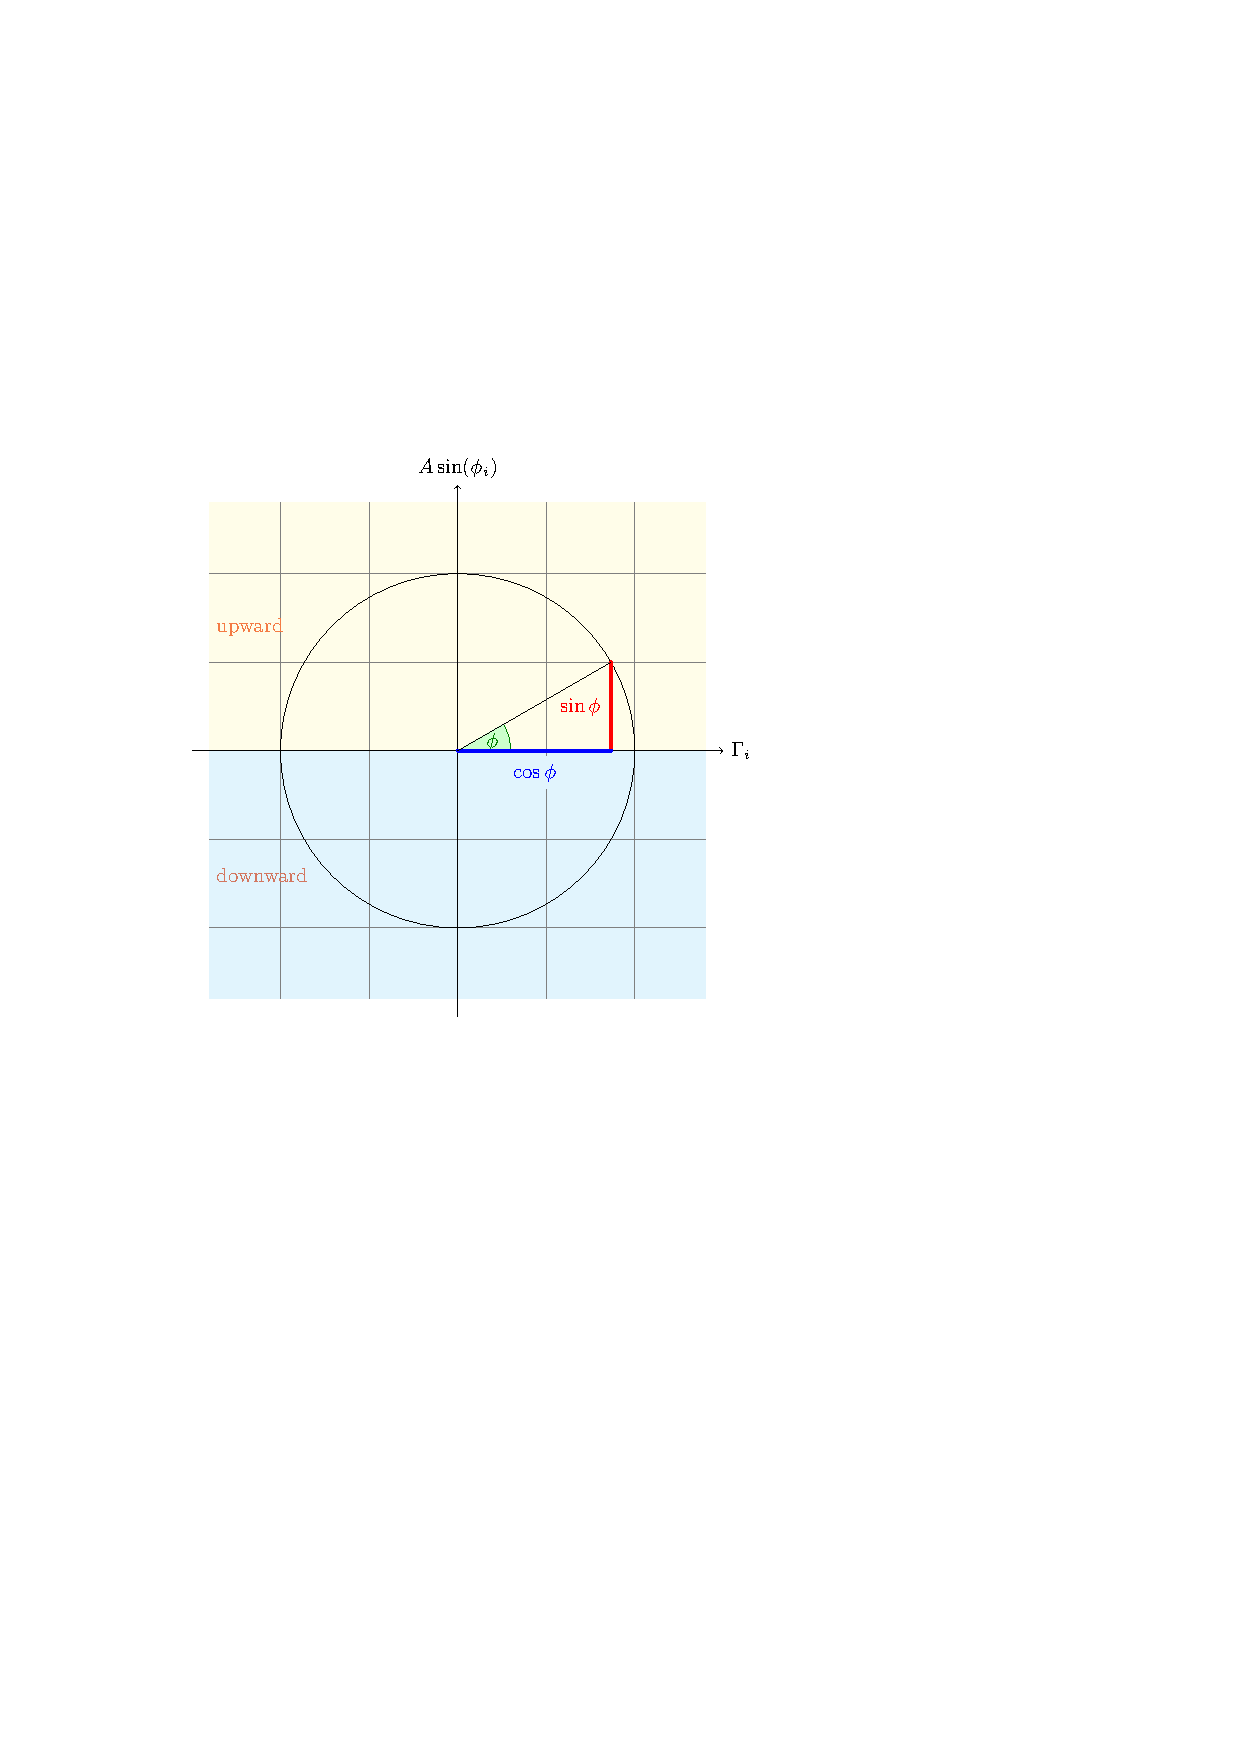
\includegraphics[scale = 0.7]{phase_plot_cropped.pdf}
		\centering
		\caption{phase}
		\label{fig:phase_plot}
\end{figure}

CPG forces ($\omega^+$ , $\omega^-$) are provided by our controller. Thus, in order to build our CPG force ($\zeta_i$), we will use: 

\begin{align}\label{eq:spliting}
	\zeta_i^+ &= \frac{1}{2}[1+ \mathrm{sign}(\sin\phi)] \omega^+\\
	\zeta_i^- &= \frac{1}{2}[1- \mathrm{sign}(\sin\phi)] \omega^-\\
	\zeta_i &= \zeta_i^+ + \zeta_i^-
\end{align}



\end{document}
